% \setchapterstyle{kao}
\setchapterimage[6.5cm]{tech_2}
\setchapterpreamble[u]{\margintoc}
\chapter[银幕背后的魔法:人工智能技术]{银幕背后的魔法:人工智能技术\footnotemark[0]}

\footnotetext{The credits for the image above the chapter title go to:
	Image generated by OpenAI's DALL-E, used in accordance with OpenAI's terms and conditions.}

随着ChatGPT模型的爆火,人工智能技术受到社会各界越来越多的关注,大家开始注意到这些应用在不同领域的人工智能算法。人工智能技术的核心是各种各样的算法,但是人工智能算法对于大众来说比较晦涩难懂,需要比较高的数学基础和编程实践能力,而且不同领域的人工智能算法具有比较大的差异,有些算法注重理论,而有些算法则脱胎于工业实践。这加大了人工智能算法的理解难度,也给人工智能技术的介绍带来了一定的困难。为了便于大众的理解,并契合本书的主题,这一章节介绍的人工智能技术的相关算法与实际产业应用和现实生活更加接近。在这一章节,为了激发大家的阅读兴趣,每个章节都会以一些经典或热门电影作为切入点,介绍隐藏在其背后的人工智能技术。

\section{《星际迷航》:语言交融的星际幻梦}

语言是我们日常交流传达信息的载体,历史上不同的国家和民族创造了不同的语言。目前的研究表明,语言的起源与人类进化过程中的社交需求密切相关。随着时间推移和社会变迁,语言也在不断地进行演变,到目前为止,世界上存在着数千种不同的语言,每一种语言都代表了特定文化和群体之间的交流方式,承载着特定文化的价值观、文化传统。另一方面不同的语言也有不同的语法结构和表达形式,这对于不同语言和文化的人之间的交流也造成了一定的困难。

而在《星际迷航:无限太空》中,演员James Doohan首次设计了克林贡语的若干基础词汇及其发音;此后逐渐有越来越多的克林贡语表达在荧幕中出现。之后1985年,美国语言学家Marc Okrand在既有的单个表达的基础上,系统地创制了整套的克林贡语单词和语法,并将之出版在其著作TheKlingon Dictionary中,至此,作为一门完善人造语言的克林贡语的雏形,得以初步确立。在剧中的太空环境下,星舰之间的通信是通过一种名为“次空间通信”的技术实现的。这种通信形式允许以超光速进行数据传输,使得在星际间发送信息成为可能。而人类与瓦肯人之间的语言存在很大差异,造成的交流障碍可以通过人工智能子领域中的自然语言处理来解决。

《星际迷航》中的次空间通信概念可以被视为自然语言处理(NLP)和机器翻译(MT)的高级形式。这些都是人工智能的子领域,专注于通过自然语言实现计算机与人类的交互。目标是使计算机能够以有价值的方式理解、解释和生成人类语言,并实现不同语言之间的互相转换。其中瓦肯人的克林贡语和英语,汉语等人类语言存在较大差距。剧中人物交流使用了一种名为万能翻译器的交流工具,保证说不同语言的人物之间的流畅交谈。

\begin{marginfigure}[-5.5cm]
	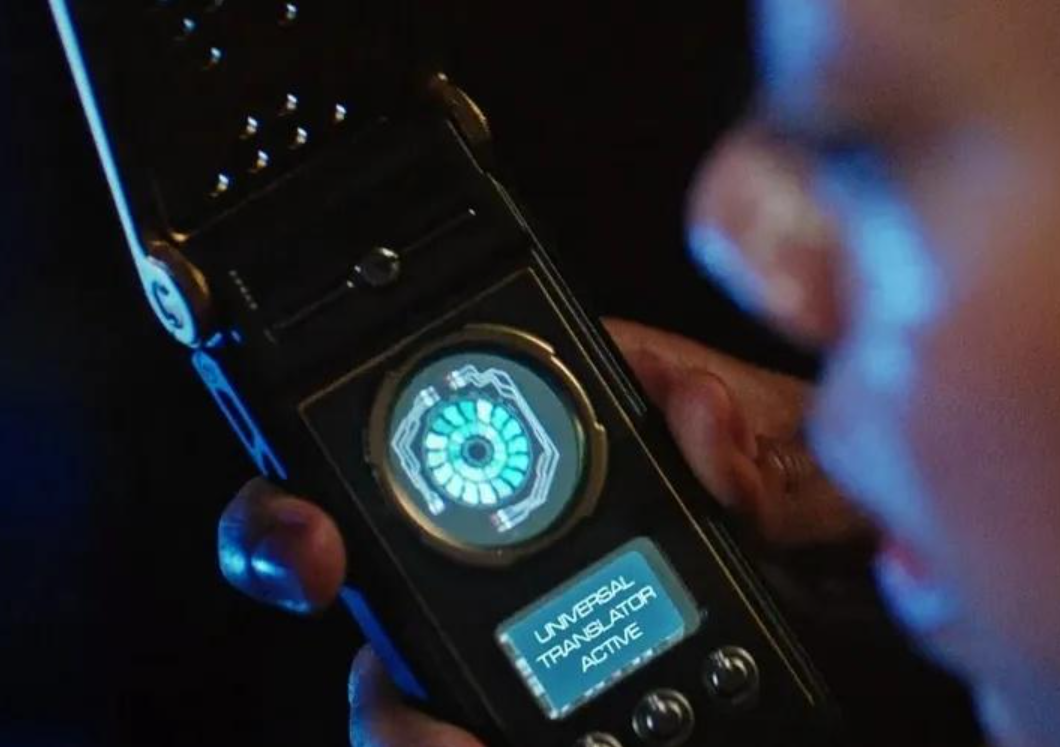
\includegraphics{tech_3.PNG}
	\caption[《星际迷航》]{《星际迷航》}
\end{marginfigure}

柯克和他的船员经常使用这种万能翻译器,可以立即将外语翻译成人类语言,使他们能够与他们在银河系中遥远星球上遇到的各种外星种族交流。实际上,目前人类并没有发现外星文明,也无法使用万能翻译器翻译外星语言,但是,这种“万能翻译器”其实在现实中已经实现了,谷歌翻译和DeepL翻译器已经实现了大部分语言的即时互译,这种翻译技术是如何实现的呢?接下来本书将从历史发展,技术原理等方面介绍机器翻译技术。

\subsection{翻译的起源}

\begin{figure}[htbp]
	\hspace{11cm}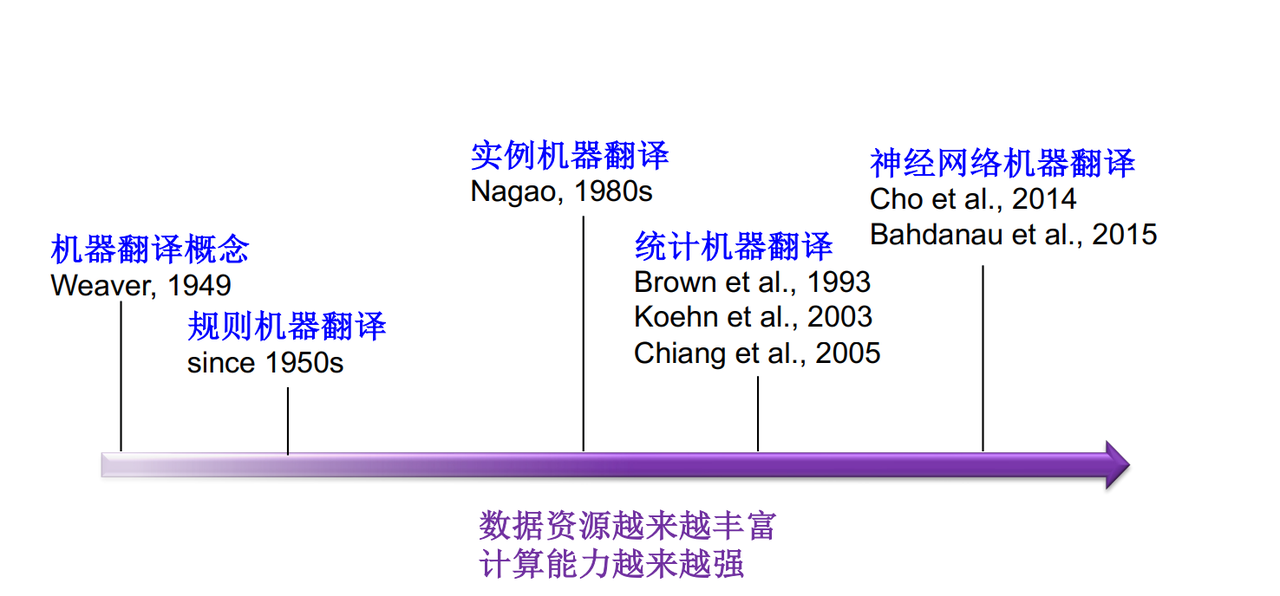
\includegraphics{tech_4.PNG}
\end{figure}
在古代,由于交通不便,文明之间的交流比较少,一般是由边境杂居通晓两种语言的人担任翻译;在交战或和谈时,国家选派的外交使臣一般也可以作为翻译官。然而这种翻译效率较为低下,无法很好地完成信息传递。随着技术的进步,计算机被科学家制作出来,紧接着在1954年乔治城大学的科学家们成功将60多条俄文句子翻译成英文,标志着机器翻译的开始。虽然当时这些句子是经过实验人员精心挑选的,但依然展示了计算机在语言翻译方面的潜质。后来,学者们经过不断钻研,提出了各种各样的翻译方法,使得机器翻译技术的效果越来越好,接下来本书会按照方法特点以及提出先后分三阶段进行介绍。

\subsection{基于规则与实例的机器翻译}
\begin{marginfigure}
    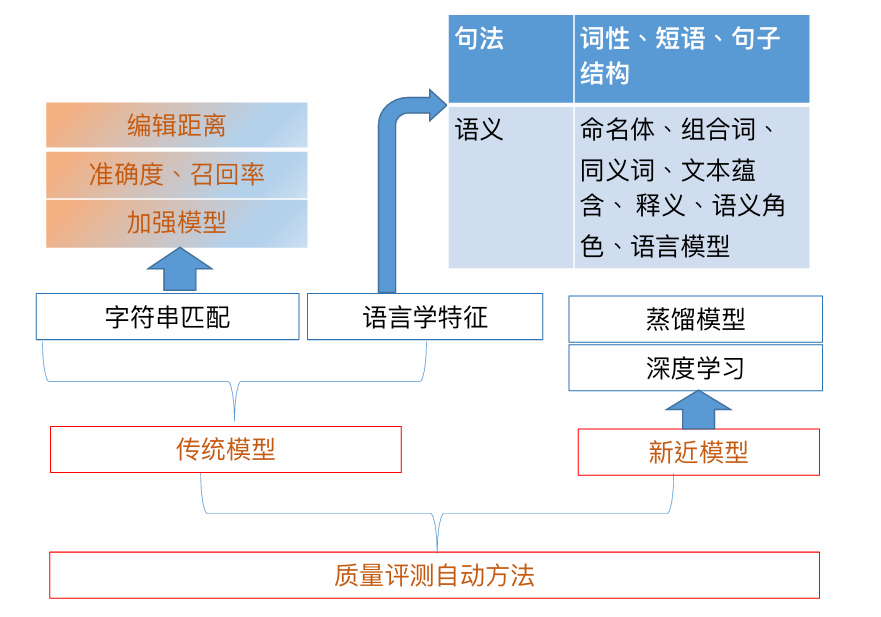
\includegraphics{tech_5.PNG}
\end{marginfigure}
第一阶段是基于规则的技术,每种语言都有自己的语言范式,我们需要理解语言的含义才能做好翻译。通过对语言结构和句法规则的理解,翻译员才能够将陌生语言的含义正确地表达出来,但这引出了一个问题,如何能够通过较低的代价深入地分析语言的共同特性?众所周知,人类的本质是复读机,自然而然地人们想到通过借鉴实例的方式进行翻译,但语言是复杂的,实例数量过于巨大,检索过程会很耗时;而且一些新词汇或陌生的语言会遇到检索不到的问题,所以这种方法现实不可行。

那要怎么办呢?既然语言都有底层的逻辑和规则,我们就可以找语言学家制定规则,翻译的时候根据规则操作就可以更加流畅地进行翻译了,那这些规则包含哪些要素呢?一般来说,规则会包含用法和词典两部分,以中英文为例,词典是英文单词与中文汉字的对应(“我”:“me”(宾语),“I”(主语)),用法是句法结构的对应(汉语主谓宾→英语主谓宾)。一个规则系统通常会包含上万条基本词典、领域词典以及人名地名词典;数千条句法规则和生成规则;并给出数万条翻译实例。制定规则的过程需要深入理解两种语言的内在结构和特点,同时也需要考虑到语言的灵活性和变化性。因此,这通常需要语言学家、翻译专家和计算机科学家的共同努力。但规则又会面临以下的问题:出现新的词语,需要扩大词典;出现新的规则,需要加入规则的同时保证不与原始规则冲突,这些更新都需要专家进行,维护难度会很大。

\subsection{统计机器学习}

随着数据资源越来越丰富,计算能力越来越强,学者们尝试新的思路进行机器翻译。既然数据资源变得越来越丰富,那么我们可以收集数据,对数据中的规律进行总结,并根据总结的规律进行翻译,于是统计机器翻译应运而生。统计机器翻译的基本流程包括以下几个步骤:第一步:预处理,将源语言和目标语言的语料库进行预处理,包括分词、词性标注等。第二步:词对齐,构建源语言和目标语言之间的词汇对应关系矩阵,以及句子之间的翻译概率矩阵。第三步:模型训练,基于构建的矩阵,使用统计方法训练机器翻译模型。第四步:翻译生成,给定一个待翻译的源语言句子,利用训练好的模型生成目标语言的翻译。

统计机器学习的核心是概率模型的选择和优化。落到机器翻译领域,统计机器翻译主要使用短语对齐模型和基于短语的统计机器翻译模型。短语对齐模型通过分析源语言和目标语言之间的词汇对应关系,找出短语级别的翻译对应关系。基于短语的统计机器翻译模型则在此基础上,通过最大熵模型或者条件随机场模型,学习出短语之间的翻译概率,其中概率模型句子的生成采用训练数据上的极大似然估计,选取概率最大的词语组成翻译。但该方法流程比较复杂,翻译性能遇到瓶颈后很难大幅度提升。


\subsection{神经网络机器翻译}
\begin{marginfigure}
    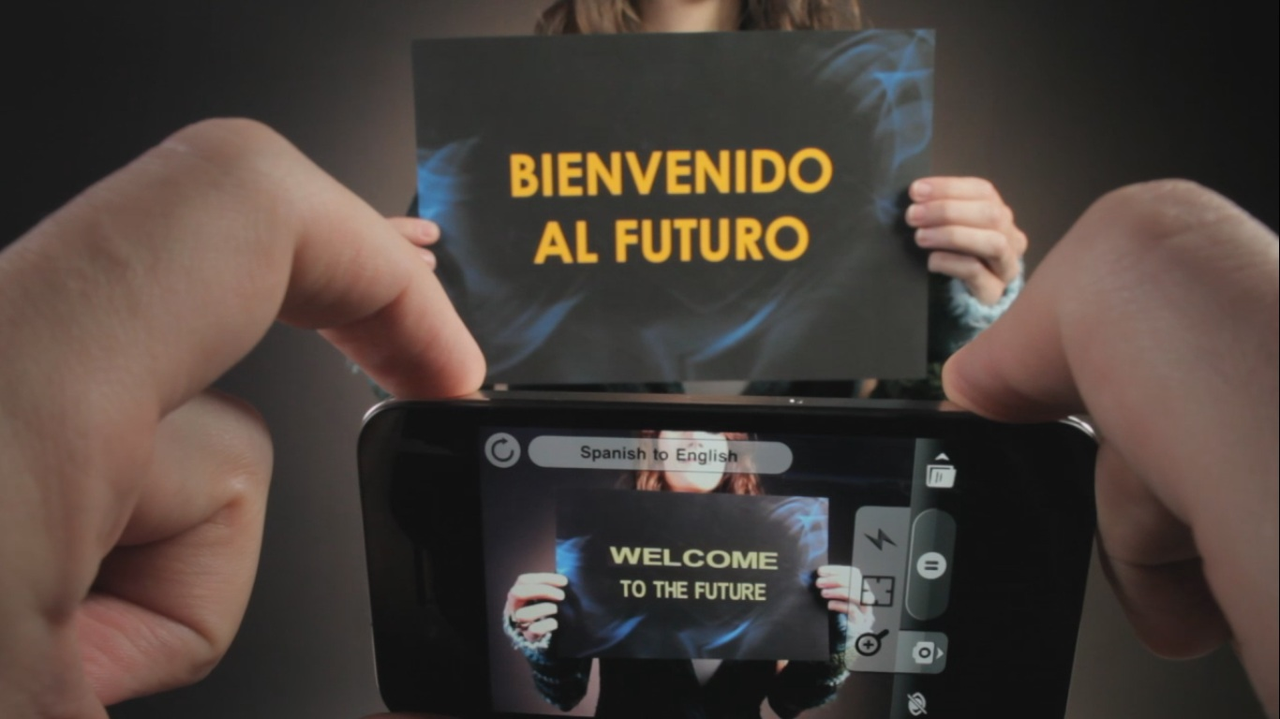
\includegraphics{tech_6.png}
\end{marginfigure}
随着深度学习技术的发展以及数据资源的进一步丰富,能够支持数据表示从符号表示转化为连续表示,机器翻译进入了下一阶段,这一阶段通常被称为神经网络机器翻译,与传统的统计机器翻译相比,神经网络机器翻译具有更好的翻译质量和更高的翻译效率。由于翻译涉及两种语言之间的转化,因此一般使用的架构是编码器-解码器架构。

编码器将源语言句子的每个单词或字符映射到一个向量空间中,这些向量表示了单词或字符的语义和语法信息。然后,编码器将这些向量组合成一个固定长度的向量,这个向量被称为编码向量。编码向量包含了源语言句子的全部信息,是解码器生成目标语言翻译的基础。

解码器则根据编码向量生成目标语言的翻译。解码器通常是一个循环神经网络,它将编码向量作为初始状态,并通过循环计算生成目标语言的每个单词或字符。在每个时间步,解码器都会生成一个单词或字符,并将生成的单词或字符和编码向量作为输入,进行下一步的循环计算。
为了提高翻译质量,神经网络机器翻译通常还需要引入注意力机制。注意力机制允许解码器在生成每个单词或字符时,根据源语言句子的不同部分来加权编码向量。这样做的好处是句子中的单词之间通常存在联系,注意力层可以隐式地学习到这种联系,从而让翻译结果更加地通顺与合理。

总的来说,神经网络机器翻译是一种比较先进的机器翻译方法,它通过神经网络和注意力机制,实现了从源语言到目标语言的高效、准确的翻译。随着深度学习技术的进一步发展,神经网络机器翻译的性能将会得到更大的提升。

\section{《头号玩家》:视觉之幻}
《头号玩家》中的虚拟现实世界是一座名为“绿洲”(OASIS)的庞大虚拟宇宙,由天才设计师詹姆斯·哈利迪创建,这部电影也是非常经典的科幻作品,其中的“绿洲”应用了虚拟现实技术、计算机视觉(CV)技术以及其他先进技术。

\begin{marginfigure}
    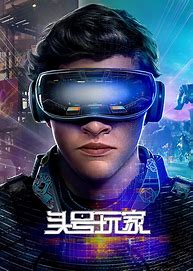
\includegraphics{images/tech_7.png}
\end{marginfigure}

\subsection{面部识别技术}

想要玩家的虚拟化身准确地反映玩家现实中的脸部表情和动作需要使用先进的面部识别技术,而且面部识别技术可以也可以确认用户身份,防止非法用户进入“绿洲”。而现实中的面部识别技术与电影中展现的技术类似,这一小节让我们来了解一下它的发展与应用。

面部识别技术是一种基于计算机视觉和模式识别技术的人脸检测和识别技术。它可以检测、识别和验证一个人的面部特征,有身份验证、安全监控、支付验证等多种用途。面部识别技术的起源可以追溯到20世纪60年代,当时采用的方案也是很朴素的数学几何特征,这集中体现在学者们对于剪影的研究上,人们对面部剪影曲线的结构特征提取与分析方面进行了大量研究,但没有收到很好的效果,也基本没有落地的应用。

\begin{marginfigure}
    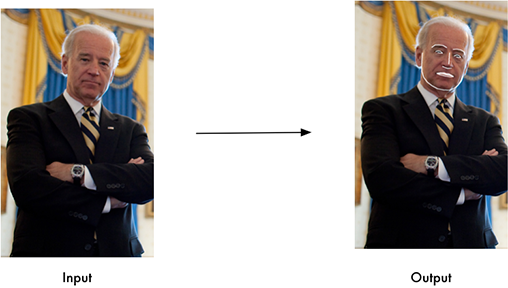
\includegraphics{images/tech_8.png}
\end{marginfigure}

突破发生在上世纪90年代,诞生了一些典型的识别技术,并产生了军事应用技术。美国麻省理工学院媒体实验室的特克和潘特兰德提出的“特征脸”方法是一种基础的人脸识别方法,之后的算法或多或少收到了该方法的影响。例如同一时期的“Fisherface”方法就有“特征脸”的思想,对输入的人脸图像进行主成分分析,提出脸部特征,然后再使用其他的算法将不同人脸的特征区分出来,达到人脸识别的效果。这一时期美国军方组织了著名的FERET人脸识别算法测试,并出现了若干商业化运作的人脸识别系统,比如最为著名的Visionics的FaceIt系统。这一时期面部识别技术蓬勃发展,不仅出现了影响后世的算法,还成功地实现了商业转化。

但这些算法会受到光照,拍到的面部表情,姿势等非理想的图片采集状态的影响,随着进入新世纪,机器学习模型的发展,支持向量机,弱分类器组合以及神经网络技术被应用于面部识别应用场景中,缓解了由于图片采集造成的识别不准确问题。近年来,随着深度学习技术的发展,面部识别技术也取得了显著的进步。深度学习技术可以提取更加丰富的面部特征,并通过神经网络进行特征匹配,从而提高面部识别的准确性和鲁棒性。目前,深度学习技术已经成为了面部识别技术的主流方法。目前卷积神经网络是面部识别技术使用最多的算法,它的主要优势是可用大量数据来训练,从而学到对训练数据中出现的变化情况稳健的人脸表征,而且不需要设计对不同类型的类内差异的特定特征。

\subsection{动作捕捉技术}

“绿洲”中虚拟角色的运动可能使用了动作捕捉技术(以下简称动捕)来模拟现实中玩家的具体动作,从而增强真实感。同样地在现代电影的拍摄过程中,动捕也是一项非常重要的辅助技术。但从宽泛的角度出发,动捕是一个非常通用的概念,它的目标可以是人体运动、面部表情、物体运动以及个体的局部信息等。动捕的起源很久远,最早是动画师发明的动作转描技术,代表作有迪士尼1937年的《白雪公主与七个小矮人》,以及1941年的《铁扇公主》和1958年的《白蛇传》。从1980年代开始,机器类的动捕设备(穿戴式)开始研发并投入使用,任天堂和麻省理工也提出了各自的光学动捕系统。

近年来,随着计算机视觉技术的发展,动作捕捉技术也取得了显著的进步,例如可以利用深度学习技术来提高动作捕捉的准确性,并将其应用于游戏开发、虚拟现实等场景。此外,动作捕捉技术也可以应用于机器人控制,以实现机器人的自主运动。国内也不乏高质量的动作捕捉系统,像诺亦腾、自然动点、青瞳视觉还有国承万通等等。另外,这几年虚拟主播的崛起使得动捕技术的应用变得更加的广泛,结合动作与面部表情的生成,主播的虚拟形象正在变得越来越精致。

\subsection{拓展现实技术}
在电影《头号玩家》中,拓展现实技术主要体现在虚拟现实(Virtual Reality, VR)和增强现实(Augmented Reality, AR)的应用上,这两种技术共同构成了电影中的“绿洲”(OASIS)世界。

虚拟现实技术在电影中表现为:人们通过佩戴高级的VR头盔(OASIS头盔)和全身跟踪设备,完全沉浸在绿洲这个虚拟世界中。他们可以在绿洲里自由移动,体验各种场景,如游戏、冒险、社交等。而通过游戏冒险等开放式挑战,绿洲将平时在电脑或手机中的游戏拓展到一个近似现实的空间中,玩家能够沉浸式体验各种冒险挑战。另一方面,虚拟环境也提供了虚拟社交平台,玩家可以在虚拟环境中与其他玩家互动,包括聊天、组队、深层次的友谊,甚至结成虚拟伴侣。此外,在类似绿洲的虚拟环境中,玩家也可以进行虚拟形象设计,发挥各自想象力,创造出千奇百怪的虚拟人物形象,甚至定制外观和能力,以展现玩家的个性。

\begin{marginfigure}
    
\includegraphics{images/tech_9.png}
\end{marginfigure}

而增强现实技术表现在现实生活中虚拟形象的投影,电影中的韦德在与虚拟角色进行对话时,利用增强现实技术可以在现实中展现角色的形象,使双方交流更有真实感。而在某些场景的虚拟现实设备启动时,韦德需要增强现实设备进行控制,比如使用类似智能手机的设备启动VR眼镜等设备,体现了增强现实技术在交互过程中的应用。

这些拓展现实技术的起源能够追溯到上个世纪60年代,其中1968年,Ivan Sutherland和他的学生Bob Sproull开发了头戴式显示器(达摩克利斯之剑),被认为是第一款现实中的AR/VR设备。上世纪80年代,3D眼镜被发明出来,并由StereoGraphics公司进行了生产,但直到本世纪,3D眼镜才逐渐流行开来。而拓展现实技术真正进入大众视野是在20世纪90年代,这一时期虚拟现实游戏机,VR眼镜,家庭VR设备陆续被各大公司创造出来,使拓展现实技术实现家庭或个人应用成为可能。而同期军事和工业领域也开始应用VR技术进行模拟实验,拓展了虚拟现实技术的应用空间。

本世纪初,随着移动设备的普及和计算能力的提升,AR技术开始逐渐被应用到手机APP中,如谷歌眼镜就是这一时期的代表。2016年,随着Pokemon Go的全球流行,AR技术进一步走进公众视野。VR技术也在这一时期获得了显著发展,代表设备有Oculus Rift、HTC Vive和PlayStation VR等。近年来,随着5G网络、AI、云计算等技术的发展,拓展现实技术正在加速走入日常生活,应用涵盖教育、医疗、工业、娱乐各个领域。未来,随着技术的不断进步,拓展现实技术有望带来更多的创新应用和体验。

虽然拓展现实技术如此的美好,但也有一些潜在的隐患。当虚拟现实能够以假乱真的时候,我们真的能够分辨出自己所处的地方到底是现实的还是虚拟的吗?游戏中的生活再美好终究也是虚假的,游戏中的你再强大,依然改变不了现实中“人被杀就会死”的真理。正如电影中的主角那样,在完成终极任务后,他终于找到了真正的自我,感悟到世间的真实情感,意识到“绿洲”不是逃避糟糕现实的避难所,面对挫折不能一味逃避而要勇于面对。最后,韦德在掌管了“绿洲”所有权后宣布,每个星期将有两天关闭“绿洲”,鼓励人们更多地体验和感受真实的生活。技术是为人类服务的,我们需要有正确的认识,并合理地使用这些技术,才能让真实的生活更加美好。

\section{《钢铁侠》:音声的魔法}

\begin{marginfigure}
    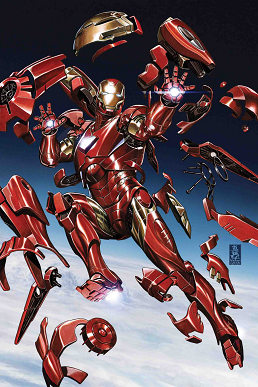
\includegraphics{images/tech_10.png}
\end{marginfigure}

贾维斯作为托尼的得力AI助手,在电影中给观众留下了很深的印象。虽然它的名字原意为”只是一个相当聪明的智能系统“,但显然这个智能系统会的技能有点太多了。它的能力包括但不限于连接到任意计算机终端;操控斯塔克的房屋和钢铁侠战服的内部系统;与托尼进行交谈以及开车等等。贾维斯其实代表了一种高度智能的语音识别和交互技术,将电影中的科技元素推向了新的高度。那么贾维斯具体包含了哪些人工智能技术呢?下面就为大家一一介绍。

\subsection{语音识别技术}

在电影中该技术具体表现为:贾维斯能够准确识别托尼的语音命令,无论是简单的指令,还是复杂的计算机操作,它都能迅速理解和执行。而现实中存在的语音识别技术需要我们输入音频(语音或对话),然后模型生成对应的文字信息。然而,我们人类经历了几百万年的进化才形成了丰富的语言系统,而且需要后天的学习才能真正掌握发音和语法,从而听懂他人的话语,表达自己的观点。那么像贾维斯这样的AI系统是如何识别我们人类的语音呢?接下来,让我们从语音识别技术的起源讲起,了解这一技术近百年的发展历史吧。

回顾语音识别技术的历史,其起源可追溯到20世纪50年代,那时的科学家致力于探索如何将口头语言转化为计算机能够处理的文本形式。此时,美国的贝尔实验室已经开始研究语音识别技术。到了60年代,贝尔实验室开发了一个名为“AUDREY”的语音识别系统,该系统可以识别数字和简单的单词。这个系统使用了手工设计的规则来匹配语音特征和词汇,然而该系统对特定人的声音特别依赖,难以适应不同的说话人的语音。随着技术的进步,70年代第一代语音识别系统开始出现,这些系统主要使用了规则引擎和手工设计的特征提取方法来实现语音识别,但这样的系统准确率相对较低,且无法识别不同的语音特征和语言,具有很大的局限性。

到了1980年代,隐马尔可夫模型(HMM)被引入到语音识别中,大大提高了识别的准确性,使得系统能够识别更复杂的词汇和短语。尽管这些系统在特定词汇集上的表现有所提升,但对连续语音和自然语言的理解能力仍然有限。1990年代,随着大规模语料库的收集和计算能力的提升,语音识别技术开始进入实用阶段。微软的“Microsoft SAPI”是这一时期的代表,win95支持该模块的运行,而且在90年代,微软一共推出了SAPI 1-4一共4个版本的API,升级了对口语以及不同程序语言的支持,应用场景也变得越来越广。

本世纪初,随着数据量的增加,深度神经网络(DNN)开始被应用于语音识别,极大地改善了识别效果。深度学习的引入使得系统能够自动从大量数据中学习特征,从而能够适应不同人的音色以及不同的语言,这是一个巨大的飞跃。研究者如Geoffrey Hinton和他在多伦多大学的团队推动了深度学习在语音识别中的应用。2011年,IBM的“Watson”在电视问答节目“危险边缘”中击败了人类选手,展示了深度学习在理解自然语言和语音识别上的潜力。谷歌、微软、亚马逊等科技巨头也纷纷推出基于深度学习的语音识别服务,如谷歌的“Google Speech API”和亚马逊的“Amazon Transcribe”。

近年来,随着硬件和云计算的快速发展,语音识别技术已经广泛应用于智能手机的语音助手、智能家居、自动驾驶汽车和医疗诊断等领域。未来,随着人工智能的进一步发展,语音识别将更加智能化,能够更好地理解语境、情感和意图,为人类带来更为便捷的交互体验。

\subsection{语音合成技术}

与语音识别技术相对应的是语音生成技术,虽然电影中的贾维斯可以聘请配音演员进行配音,但现实中的AI对话不可能找演员进行实时配音。此时我们需要一个可以生成语音的模型帮助我们生成需要的声音,一般情况下,此类模型需要的输入为声音对应的文本数据,可以是简单的单词、句子、段落或完整的文档,在应用的时候可以是用户输入的命令、文章内容、电子书文本等;另外,有些模型也可以输入一些要求,比如:语气的轻重缓急,重音位置,声音性别等个性化需求。对应的输出一般为音频流,有实时的语音信号或者保存为MP3,WAV等格式的音频文件,以便用户的存储和播放需求。从这个角度来说,语音合成技术通过将文本转换为可听的语音,实现了信息的无障碍传递,为视觉障碍人士、语言障碍人士以及有阅读困难的人提供了极大的帮助。

而语音合成技术的起步甚至比语音识别技术更早,在1930年代,科学家开始探索通过机械和电子设备生成语音的可能性,但并没有什么实质性的成果。到了1962年,有实验室展示了他们发明的可以合成语音的机器,但这时是实验人员调整机器参数,生成的声音极其有限。之后到了70,80年代,根据声学底层原理提出的一类共振峰合成器成为了主流的语音合成技术,只要实验人员精心调整参数,此类合成器能合成出非常自然的语音。而最具代表性的文语转换系统数美国DEC公司在1987年提出的DECtalk,该系统采用Klatt的串/并联共振峰合成器,可以通过标准的接口和计算机联网或单独接到电话线路上提供各种语音信息服务,它的发音清晰,并可产生几种不同音色的声音,供用户选择。

八十年代末期,语言合成技术又有了新的进展,特别是1990年研究员们提出的基音同步叠加(PSOLA)方法,该方法采用时域波形拼接的思想,使得合成的语音的音色和自然度大大提高。之后,不同语言的PSOLA方法也陆续被科学家们实现,基于这类简单的方法,可以开发出很多语音合成系统,比如中国科学院声学所的KX-PSOLA(1993),联想佳音(1995)。但这些系统合成的句子及篇章语音机器味较浓,其自然度还不能达到用户可广泛接受的程度,从而制约了这项技术的大规模进入市场。

21世纪以来,随着统计建模和机器学习算法的发展,语音合成技术开始采用隐马尔可夫模型(HMM)和波形建模等技术,使语音合成的自然度显著提高。这一时期的代表是IBM开发的可以在嵌入式设备中使用的Viavoice,该系统由6个部分组成,不仅提供了语音合成功能,也可以进行语音识别。

\subsection{情感理解技术}

该技术属于心理学和计算机科学的交叉领域,电影中的贾维斯能够理解托尼的情感,直到它“死亡”都没有背叛过托尼,具有鲜明的人物形象。但现实中该能力对AI来说是一项很有挑战性的任务,从这一技术的历史发展我们可以感受到这一技术挑战的难度。

情感理解的提出在上世纪80年代左右,当时科学家做的是情感识别工作,例如通过使用规则或统计模型分析文本中的情感词汇和语调来识别作者的情绪,显然这项任务与情感理解具有很大的差异。90年代后,研究人员开始构建情感词典,通过量化含有情感的词语的方式进行情感识别。到本世纪,科学家们又引入机器学习方法和深度学习模型进行文本情感的理解。最近十年,随着生成式模型的出现,情感反馈与生成也成为了该领域的研究热点,该任务不仅要求模型能够识别情感,还需要生成具有情感色彩的回复。

但这也产生了一个问题,AI模型是否具备自我意识,是否存在伦理与法律上的问题。虽然目前AI模型已经很大,可以完成各种各样的任务,但它们还不具备真正的自我意识。然而随着科技发展,未来的人工智能是否会拥有自我意识仍然是一个未知的事情。

\section{《流浪地球》:大模型的奇幻时代}
\subsection{科幻作品中的大模型}

\begin{marginfigure}
    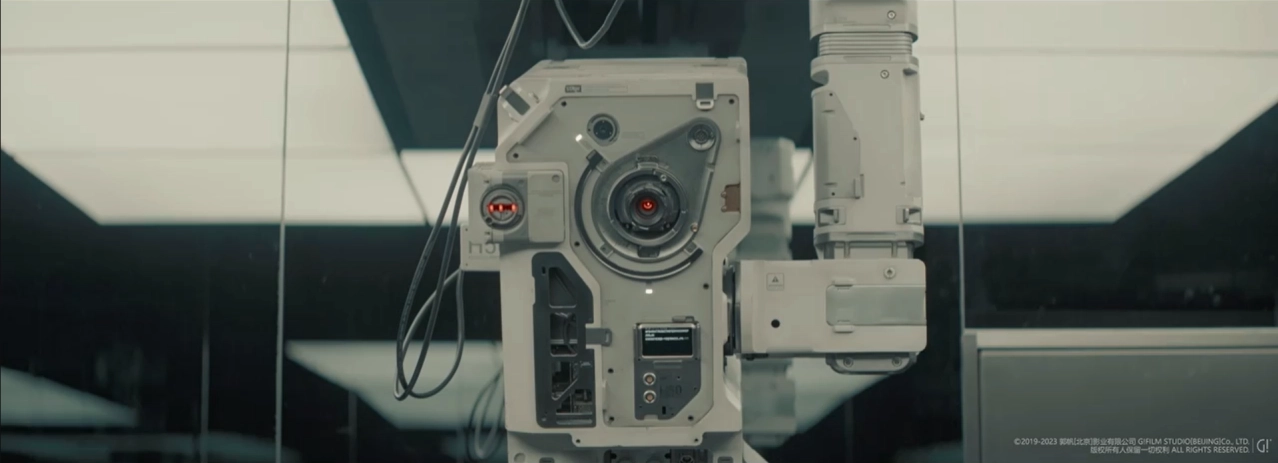
\includegraphics{images/tech_11.png}
\end{marginfigure}

在电影《流浪地球》中,MOSS是一个智能量子计算机,后因“隔离计划”被转移至领航员空间站,负责管理空间站事务,是“流浪地球”计划辅助执行者、“火种”计划的执行者,拥有联合政府授权。其拥有两种形态,其中生活仓的MOSS为白色,在总控室的MOSS是黑色。虽然在电影中MOSS算是辅助角色,但其具备的能力确实十分的强大,具有丰富的世界知识,能够进行自主学习并适应环境变化,可以进行自主决策并与主角进行流畅的对话。

虽然MOSS十分强大,但目前现实中并没有类似的AI模型拥有与之匹配的能力,如果矮子里面调将军的话,大模型算是最接近MOSS的人工智能技术。那么,什么是大模型呢?

\subsection{大模型技术介绍}

大模型目前没有一个非常明确的定义,通常指人工智能领域中,拥有海量参数的复杂模型。这些模型通常用于处理自然语言处理(NLP)、图像识别、语音识别等多种任务,能够从大量的训练数据中学习到复杂的模式和特征。大模型一般情况下使用神经网络架构(Transformer),其参数量一般可以达到十几亿甚至数千亿,这使得它们有能力学习更为精细的数据特征,并能更好地适应各种复杂的任务。由于大模型的参数量巨大,模型训练时需要的数据量也很大,而且大模型通常采用预训练的方式,通常先在一个大规模无标注的数据集上进行预训练,学习通用的语言或视觉表示。该数据集一般是收集网络上的数据后进行筛选构成的,训练时,这些数据(很多都是类似对话、文章等长序列数据)被输入给模型,随后转为词向量进行进一步的特征提取,最终大模型学到这些数据的通用表示。之后,可以根据特定任务需求在相关的小数据集上进行模型微调,以提升在特定下游任务上的性能。目前,训练大模型需要大量的计算资源,包括高性能的GPU或TPU等硬件,以及海量的数据和模型的存储空间。不过同时,大模型在自然语言理解和生成、智能助手、自动翻译、推荐系统等领域具有广泛的应用。

\subsection{大模型的发展历史}
大模型相关技术的提出还是比较早的,上世纪50年代神经网络已经被学者们提出并进行了实验,但当时由于组成神经元的参数过少,数据量不足等原因,神经网络的效果比不过专家系统和规则方法。因此神经网络方法沉寂了约40年的时间,直到1980年代,卷积神经网络(CNN)的雏形出现,为图像识别和计算机视觉领域带来了新的突破,之后在1990年代末,现代CNN的基本结构LeNet-5被提出,深度学习技术开始崭露头角。

随着自然语言处理技术的发展,词向量模型被提出,标志着大模型的部分底层技术逐渐成形。2017年,Google提出了Transformer模型,该模型以其自注意力机制和并行处理能力,为处理长序列数据提供了新的方法。2018年,GPT-1和BERT模型的发布,开启了预训练模型的时代。

随着技术的积累和数据量的增加,模型参数量变得越来越大,2020年,OpenAI的GPT-3(Generator Pre-training-3)模型横空出世,拥有1750亿参数,成为当时最大的语言模型。此时,模型的参数规模达到了前所未有的水平,为零样本学习(可以理解为没有模型微调阶段)和自然语言处理带来了巨大进步。同时研究人员在训练GPT-3时也使用了一些新提出的技术,如基于人类反馈的强化学习(RLHF)和代码(编程语言)预训练。

等会,我们介绍了那么多,怎么还没有大模型这一概念呢?事实上,大模型这一概念是很多人工智能技术综合的产物,直到22年底OpenAI提出ChatGPT模型并引发广泛关注,通常意义上的大模型才出现在大众的视野,由于模型参数量变得很大,这一类的模型被称为“大模型”,其自然语言交互能力在多个领域展现了巨大潜力。另一方面,随着视觉-语言模型如CLIP(Contrastive Language-Image Pretraining)和DALL-E的推出,研究人员开始整合视觉和语言信息,并提出可以处理多类输入信息的大模型。

在国内,产业界、投资界和研究机构等都在投身大模型研究。首先,国内科技龙头企业纷纷发布自主研发的大模型,比如百度推出了大模型文心一言,阿里巴巴发布了大规模语言模型通义千问,智谱AI也率先进行了商业化的落地,推出了不同参数量级的商业化模型ChatGLM系列。这些竞争促进了大模型社区的良性发展,目前世界范围内呈现出“百模齐放”的景象,出现了兼容不同语言,不同模态的大模型。

大模型的发展不仅推动了人工智能技术的进步,也在实际应用中产生了深远影响,如智能助手、自动翻译、推荐系统等。目前,研究人员也在积极探索大模型在生物医学,化学制造等方面的应用,包括但不限于制造化学分子,进行化学实验,模拟生成人工蛋白质等。
